\section{Background and Information}\label{background-and-information}

\subsection{Verbal Fluency and SpAM
Context}\label{verbal-fluency-and-spam-context}

The verbal fluency task asks participants to type category words in
limited time. SpAM asks participants to place words in 2D space based on
semantic similarity. This project combines both tasks in Hindi.

Main goal is to check if semantic structure from SpAM is reflected in
retrieval timing from VFT.

\subsection{Research Questions}\label{research-questions}

{\def\LTcaptype{none} % do not increment counter
\begin{longtable}[]{@{}
  >{\raggedright\arraybackslash}p{(\linewidth - 4\tabcolsep) * \real{0.1071}}
  >{\raggedright\arraybackslash}p{(\linewidth - 4\tabcolsep) * \real{0.6786}}
  >{\centering\arraybackslash}p{(\linewidth - 4\tabcolsep) * \real{0.2143}}@{}}
\toprule\noalign{}
\begin{minipage}[b]{\linewidth}\raggedright
\#
\end{minipage} & \begin{minipage}[b]{\linewidth}\raggedright
Research Question
\end{minipage} & \begin{minipage}[b]{\linewidth}\centering
Type
\end{minipage} \\
\midrule\noalign{}
\endhead
\bottomrule\noalign{}
\endlastfoot
RQ1 & Is within-cluster IRT different from between-cluster IRT? &
Confirmatory \\
RQ2 & Does mean cluster size predict total fluency? & Confirmatory \\
RQ3 & Does SpAM distance relate to VFT IRT? & Confirmatory \\
RQ4 & Is SpAM compactness different across domains? & Confirmatory \\
RQ5 & Does participant-level SpAM dispersion predict VFT switching cost?
& Confirmatory \\
EH1 & Do IRT distributions differ across domains? & Exploratory \\
EH2 & Does serial position affect IRT? & Exploratory \\
EH3 & Does code-switching pattern differ by domain? & Exploratory \\
EH4 & Which cluster metric is most related to fluency? & Exploratory \\
\end{longtable}
}

\subsection{Simple Meaning of RQ and
EH}\label{simple-meaning-of-rq-and-eh}

\begin{itemize}
\tightlist
\item
  RQ1 means: is switching slower than staying in same cluster.
\item
  RQ2 means: do bigger clusters give more words.
\item
  RQ3 means: do SpAM distances match VFT timing.
\item
  RQ4 means: is semantic compactness same in all domains.
\item
  RQ5 means: does person-level SpAM spread explain person-level switch
  cost.
\item
  EH1 means: is timing different across domains.
\item
  EH2 means: does later response position change timing.
\item
  EH3 means: does Hindi-English mix change by domain.
\item
  EH4 means: which cluster metric helps fluency most.
\end{itemize}

\subsection{Previous Work and Study
Position}\label{previous-work-and-study-position}

Previous VFT work mainly focuses on clustering and switching. Most
studies are in English and western language settings. Hindi data with
script mixing and code-switching is less studied.

SpAM work gives direct semantic layout from participant judgments. This
is useful because it gives a second view of semantic structure. Our work
combines VFT timing and SpAM distance in same participant sample.

Troyer et al.~showed clustering and switching as two key parts of
fluency behavior. Hills et al.~explained retrieval with optimal foraging
view in semantic memory. Hout et al.~showed SpAM as a useful method for
semantic similarity mapping.

Kumar, Lundin and Jones (PsyArXiv 2bazx) showed that semantic and
phonological information jointly affect retrieval in semantic fluency.
Dautriche et al.~(2016) showed in 100 languages that semantically
similar words are often more phonologically similar also.

These past studies support our design choice to combine semantic
structure and retrieval timing in one analysis pipeline.

\section{Experiment}\label{experiment}

\subsection{Participants and Design}\label{participants-and-design}

This is within-subject design. Each participant completed all four
domains.

{\def\LTcaptype{none} % do not increment counter
\begin{longtable}[]{@{}ll@{}}
\toprule\noalign{}
Variable & Value \\
\midrule\noalign{}
\endhead
\bottomrule\noalign{}
\endlastfoot
N & 35 \\
Domains & animals, foods, colours, body-parts \\
Rows in final analysis & 1044 \\
Main timing variable & rt\_ms \\
\end{longtable}
}

\subsection{Procedure Summary}\label{procedure-summary}

\begin{enumerate}
\def\labelenumi{\arabic{enumi}.}
\tightlist
\item
  Participants typed category words in VFT with timestamp logging.
\item
  Same participants completed SpAM by placing words on canvas.
\item
  Processing was done domain-wise for both tasks.
\end{enumerate}

\section{Data}\label{data}

\subsection{VFT Data Processing}\label{vft-data-processing}

\begin{enumerate}
\def\labelenumi{\arabic{enumi}.}
\tightlist
\item
  Kept valid rows and valid rt\_ms values.
\item
  Built within-cluster and between-cluster means by participant and
  domain.
\item
  Computed total fluency and cluster metrics.
\item
  Built domain-wise summary tables.
\end{enumerate}

\subsection{SpAM Data Processing}\label{spam-data-processing}

\begin{enumerate}
\def\labelenumi{\arabic{enumi}.}
\tightlist
\item
  Extracted x and y coordinates from responses.
\item
  Built participant-wise euclidean distance matrices.
\item
  Built consensus matrix by averaging valid pair distances.
\item
  Computed compactness using nearest neighbour distance.
\item
  Computed participant-level dispersion using mean pairwise distance.
\end{enumerate}

\section{Methodology}\label{methodology}

\subsection{Normality First Test
Selection}\label{normality-first-test-selection}

We used Shapiro Wilk normality check before choosing tests.

\begin{itemize}
\tightlist
\item
  If p \textgreater= 0.05 then parametric test is possible.
\item
  If p \textless{} 0.05 then non parametric test is used.
\end{itemize}

Most key variables were non normal. So non parametric tests were primary
in final inference.

\subsection{Transformer Method: What and
How}\label{transformer-method-what-and-how}

Transformer model used:

\begin{itemize}
\tightlist
\item
  sentence-transformers/paraphrase-multilingual-MiniLM-L12-v2
\end{itemize}

How we used it:

\begin{enumerate}
\def\labelenumi{\arabic{enumi}.}
\tightlist
\item
  Generated embeddings for words in each domain.
\item
  Computed cosine similarity and cosine distance between word pairs.
\item
  Built neighbourhood density feature from nearest semantic neighbors.
\item
  Tested neighbourhood density relation with rt\_ms using mixed model.
\end{enumerate}

Why this helps:

This gives model-based semantic closeness. Then we compare this with
human behavior timing. So we get computational and behavioral semantic
views together.

\subsection{Test Justification Table}\label{test-justification-table}

{\def\LTcaptype{none} % do not increment counter
\begin{longtable}[]{@{}
  >{\raggedright\arraybackslash}p{(\linewidth - 6\tabcolsep) * \real{0.2500}}
  >{\raggedright\arraybackslash}p{(\linewidth - 6\tabcolsep) * \real{0.2500}}
  >{\raggedright\arraybackslash}p{(\linewidth - 6\tabcolsep) * \real{0.2500}}
  >{\raggedright\arraybackslash}p{(\linewidth - 6\tabcolsep) * \real{0.2500}}@{}}
\toprule\noalign{}
\begin{minipage}[b]{\linewidth}\raggedright
Question
\end{minipage} & \begin{minipage}[b]{\linewidth}\raggedright
Normality status
\end{minipage} & \begin{minipage}[b]{\linewidth}\raggedright
Test used
\end{minipage} & \begin{minipage}[b]{\linewidth}\raggedright
Why this test
\end{minipage} \\
\midrule\noalign{}
\endhead
\bottomrule\noalign{}
\endlastfoot
RQ1 & paired difference non normal & Wilcoxon signed rank & paired non
normal comparison \\
RQ2 & predictor and residual non normal & Spearman correlation &
monotonic non normal relation \\
RQ3 & pairwise variables non normal & Spearman correlation & rank based
pairwise relation \\
RQ4 & compactness non normal & Kruskal Wallis + BH post hoc Mann Whitney
& multi-group non normal comparison \\
RQ5 & both variables non normal & Spearman + MixedLM & non normal
relation + repeated measure robustness \\
EH1 & domain IRT non normal & Kruskal Wallis & skewed multi-group
comparison \\
EH2 & repeated structure & Mixed model + domain slopes & repeated
measurements handling \\
EH3 & proportion pattern & descriptive proportion analysis & count-based
pattern check \\
EH4 & metrics mostly non normal & Spearman correlation & robust
rank-based relation \\
\end{longtable}
}

\section{Hypothesis Testing}\label{hypothesis-testing}

\subsection{RQ1: Within-cluster vs Between-cluster
IRT}\label{rq1-within-cluster-vs-between-cluster-irt}

\begin{itemize}
\tightlist
\item
  Test: Wilcoxon signed rank
\item
  W = 277.0
\item
  p = 0.368
\item
  Decision: Not significant
\end{itemize}

Interpretation: Switching gap is not reliably present in this sample. We
cannot claim that switching is slower in final data.

\begin{figure}
\centering
\pandocbounded{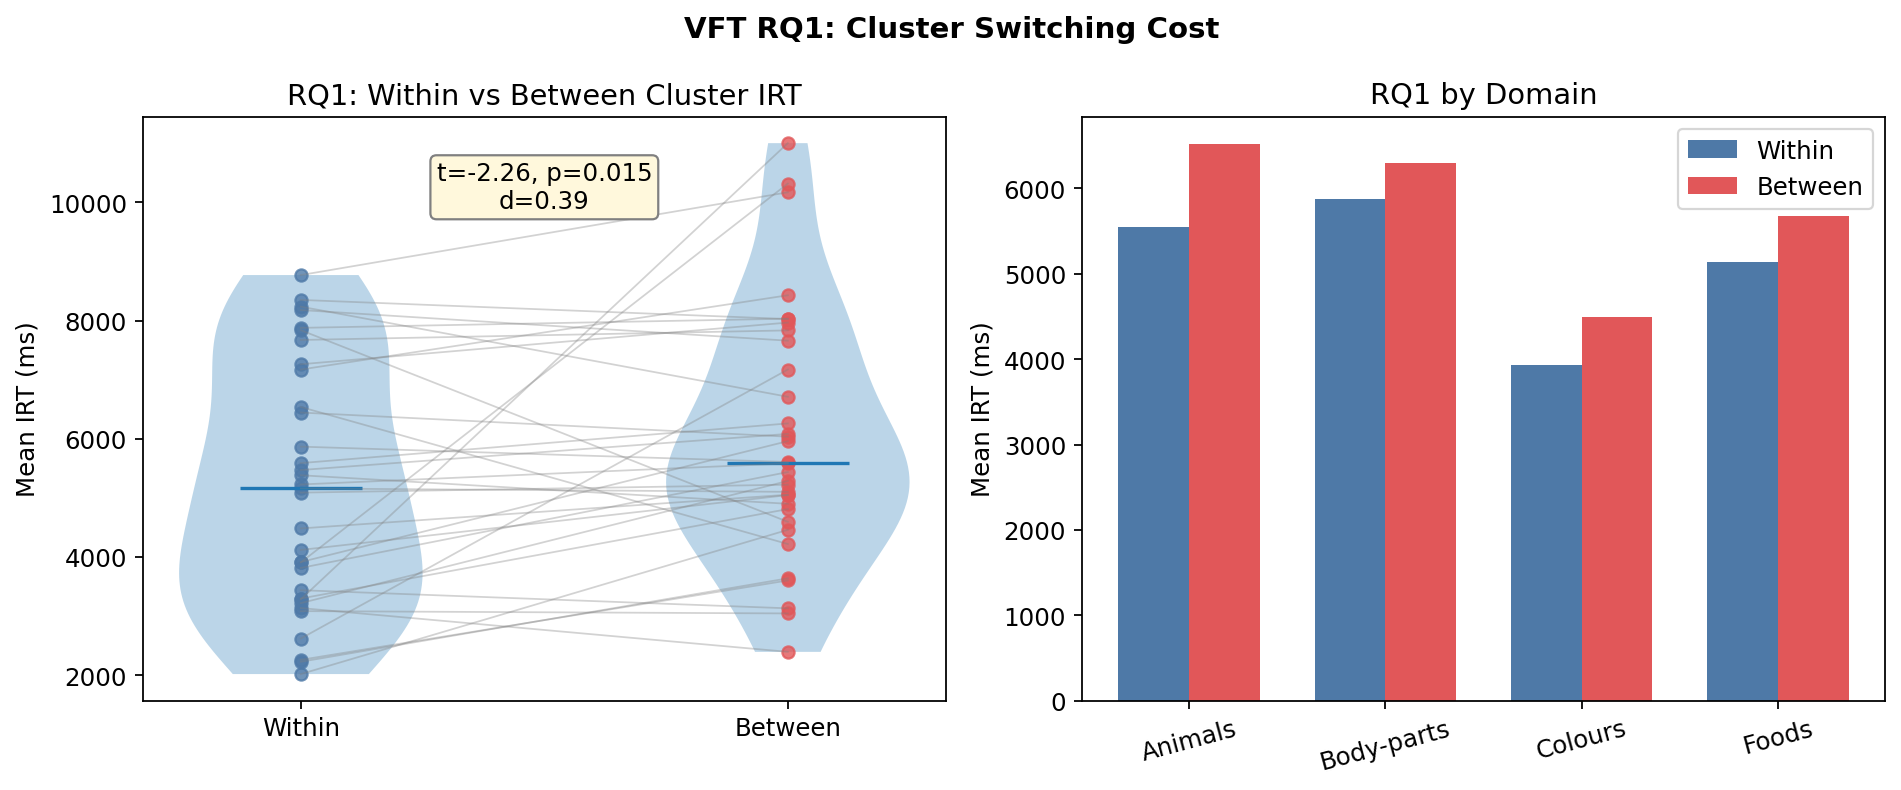
\includegraphics[keepaspectratio,alt={RQ1 within vs between}]{images/vft_fig01_rq1_within_between.png}}
\caption{RQ1 within vs between}
\end{figure}

\subsection{RQ2: Mean Cluster Size vs Total
Fluency}\label{rq2-mean-cluster-size-vs-total-fluency}

\begin{itemize}
\tightlist
\item
  Test: Spearman correlation
\item
  rho = 0.494
\item
  p = 0.003
\item
  Decision: Significant positive relation
\end{itemize}

Interpretation: Larger cluster size is associated with higher fluency
output. This suggests better semantic grouping supports better retrieval
output.

\begin{figure}
\centering
\pandocbounded{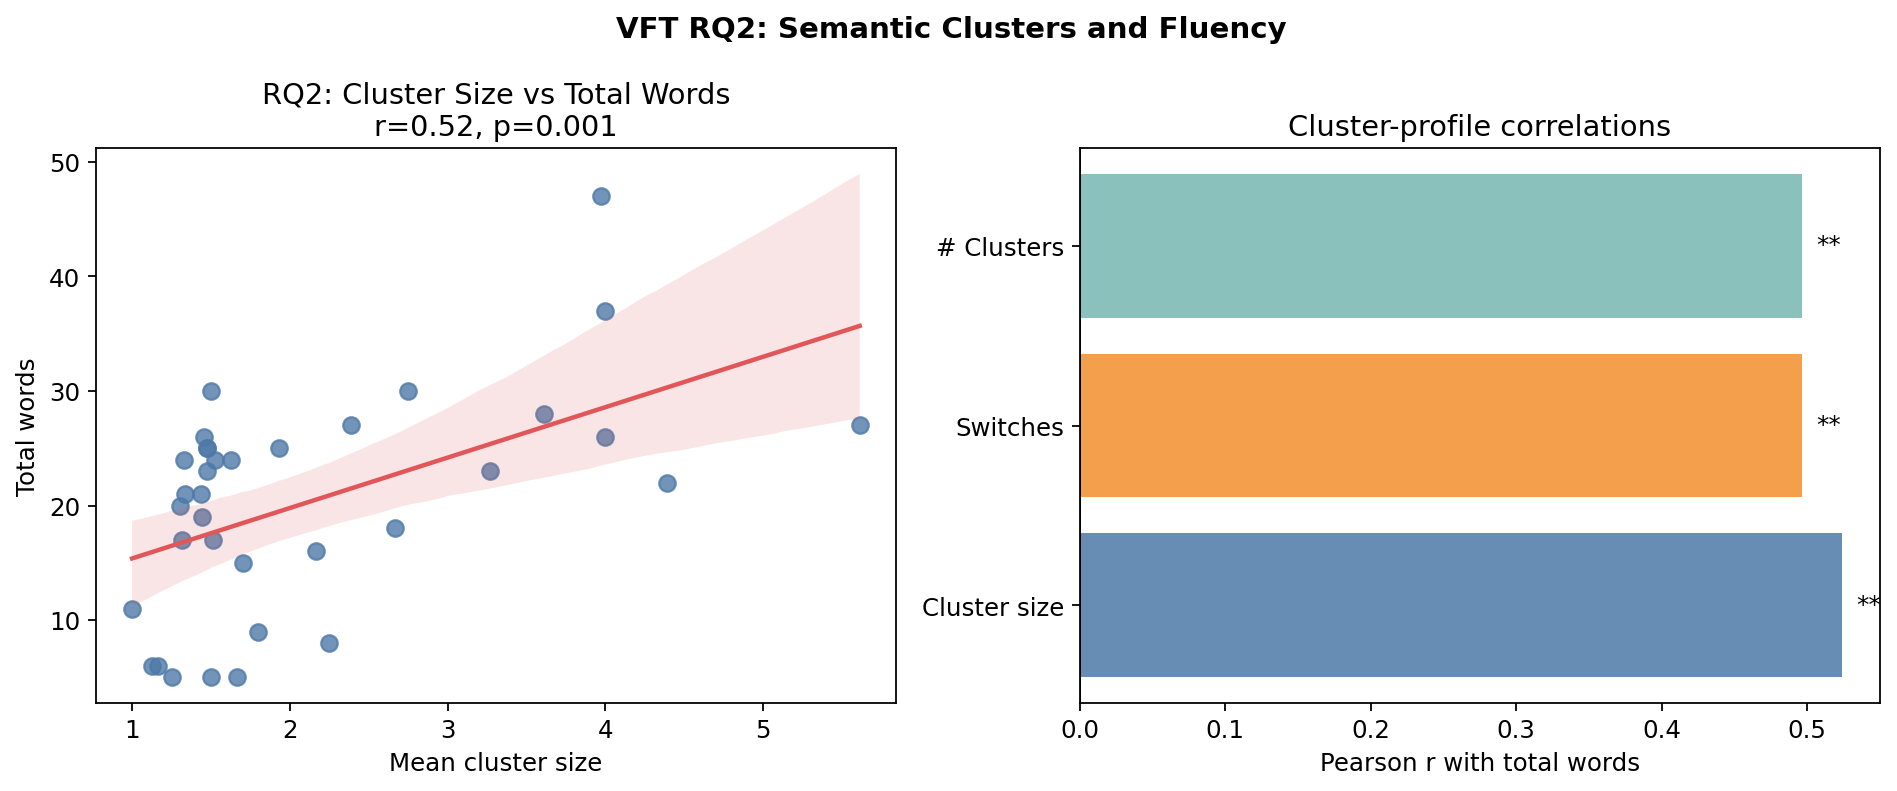
\includegraphics[keepaspectratio,alt={RQ2 cluster vs fluency}]{images/vft_fig02_rq2_cluster_fluency.png}}
\caption{RQ2 cluster vs fluency}
\end{figure}

\subsection{RQ3: SpAM Distance vs VFT
IRT}\label{rq3-spam-distance-vs-vft-irt}

\begin{itemize}
\tightlist
\item
  Test: Spearman correlation
\item
  Overall rho = -0.304
\item
  Overall p \textless{} .001
\end{itemize}

Domain-wise values:

{\def\LTcaptype{none} % do not increment counter
\begin{longtable}[]{@{}lrr@{}}
\toprule\noalign{}
Domain & rho & p \\
\midrule\noalign{}
\endhead
\bottomrule\noalign{}
\endlastfoot
Animals & -0.242 & 0.00009 \\
Foods & -0.090 & 0.345 \\
Colours & 0.080 & 0.376 \\
Body-parts & -0.111 & 0.298 \\
\end{longtable}
}

Interpretation: Cross-task relation is strongest in Animals. Other
domains are weaker in this dataset. So global signal exists but domain
pattern is not uniform.

\begin{figure}
\centering
\pandocbounded{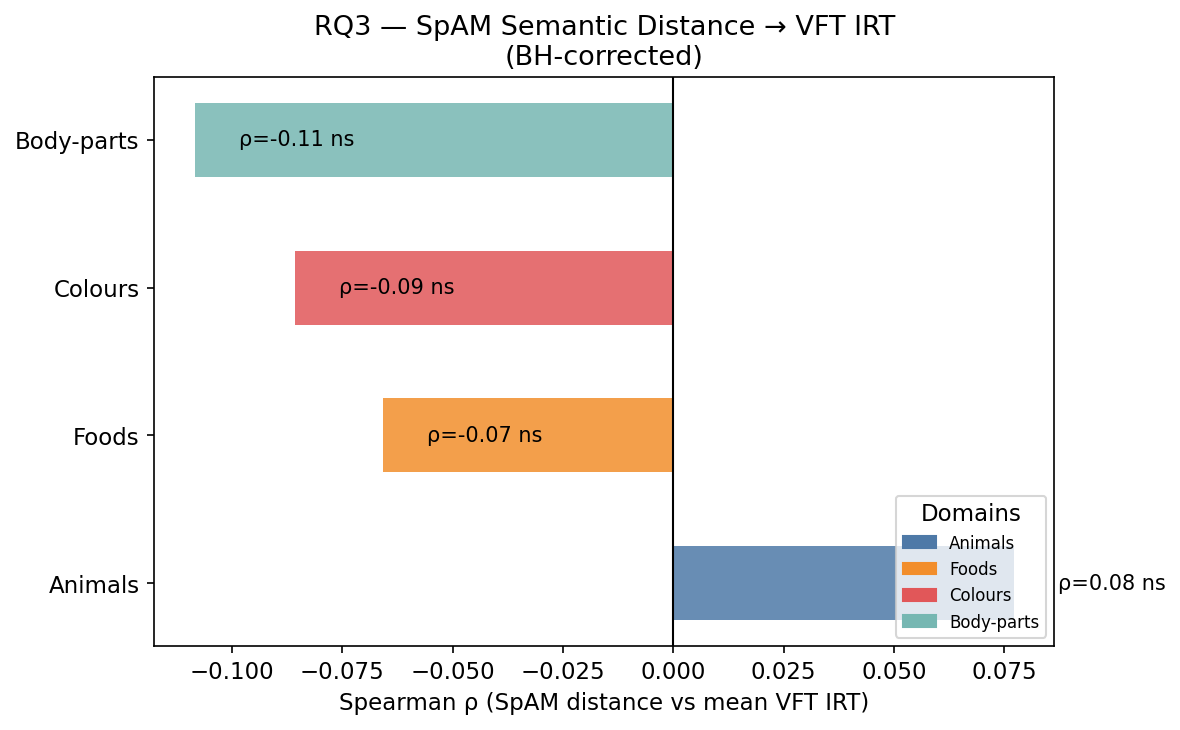
\includegraphics[keepaspectratio,alt={RQ3 SpAM vs VFT}]{images/rq3_spam_vft_correlation.png}}
\caption{RQ3 SpAM vs VFT}
\end{figure}

\subsection{RQ4: SpAM Compactness Across
Domains}\label{rq4-spam-compactness-across-domains}

\begin{itemize}
\tightlist
\item
  Test: Kruskal Wallis
\item
  H = 24.45
\item
  p \textless{} .001
\end{itemize}

Post hoc after BH correction:

\begin{itemize}
\tightlist
\item
  Colours differs from animals foods and body-parts
\item
  animals vs foods is not significant
\item
  animals vs body-parts is not significant
\item
  foods vs body-parts is not significant
\end{itemize}

Interpretation: Semantic compactness is domain dependent. Colours has
clearly different compactness profile. This supports domain-specific
semantic organization.

\begin{figure}
\centering
\pandocbounded{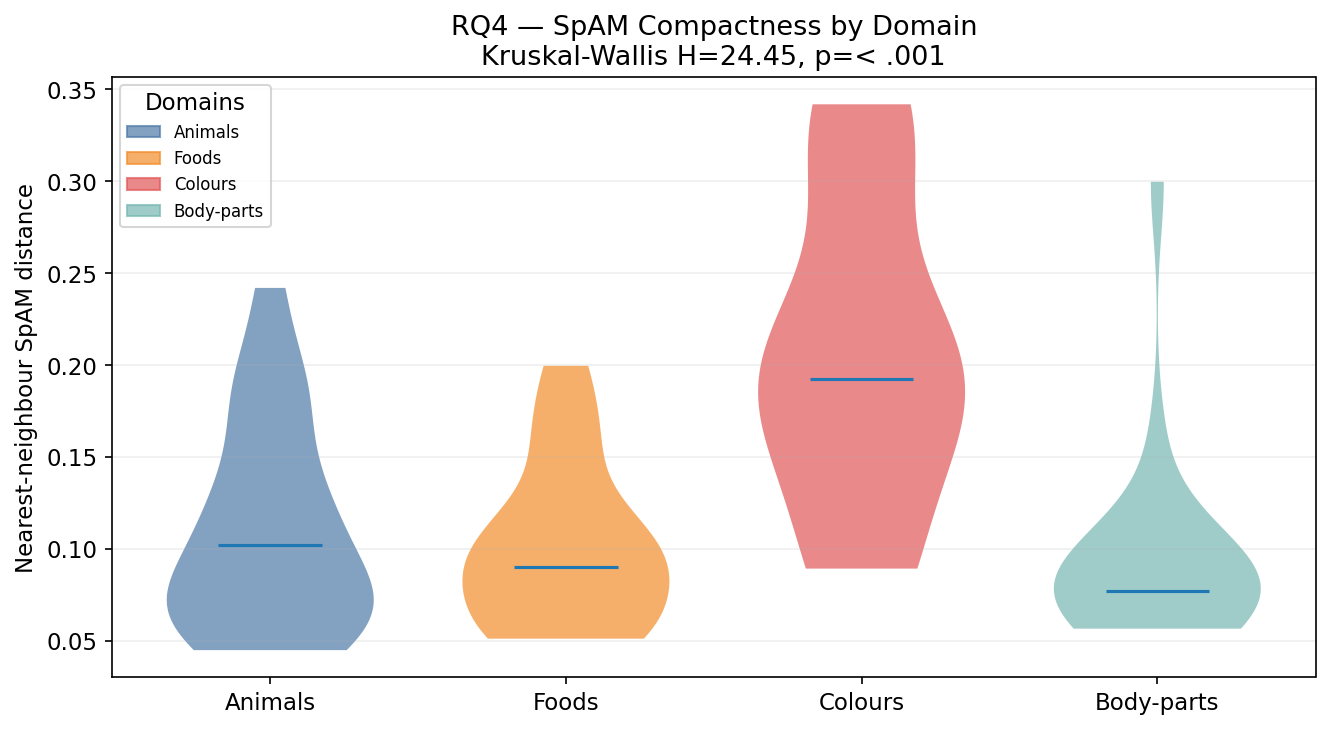
\includegraphics[keepaspectratio,alt={RQ4 compactness}]{images/rq4_spam_compactness_by_domain.png}}
\caption{RQ4 compactness}
\end{figure}

\subsection{RQ5: SpAM Dispersion vs VFT Switching
Cost}\label{rq5-spam-dispersion-vs-vft-switching-cost}

\begin{itemize}
\tightlist
\item
  Test: Spearman and MixedLM
\item
  Spearman rho = 0.01 p = 0.954
\item
  MixedLM beta = -669.7 p = 0.801
\item
  Decision: Not significant
\end{itemize}

Interpretation: Participant-level SpAM spread does not explain switching
cost. So higher map spread does not imply higher switch penalty.

\begin{figure}
\centering
\pandocbounded{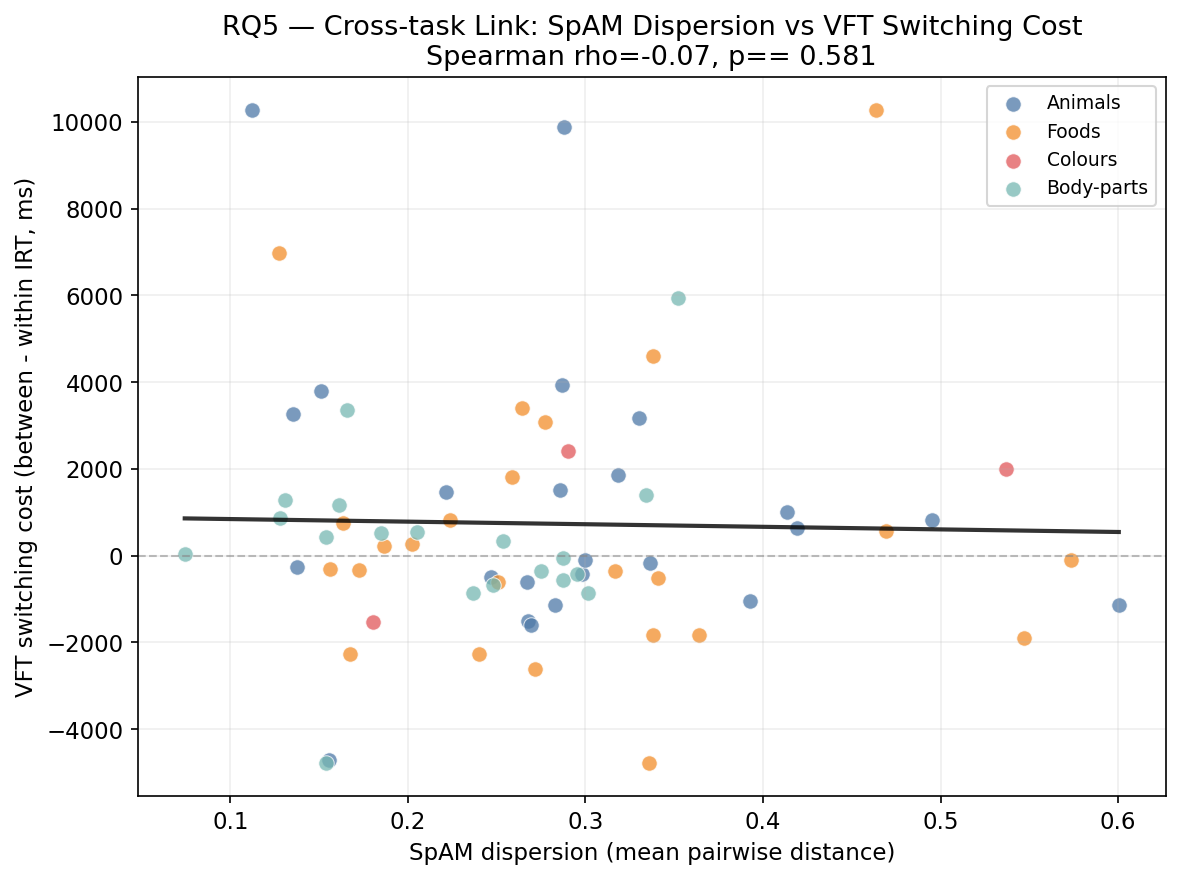
\includegraphics[keepaspectratio,alt={RQ5 dispersion vs switch cost}]{images/rq5_spam_vft_switchcost.png}}
\caption{RQ5 dispersion vs switch cost}
\end{figure}

\section{Exploratory Hypotheses}\label{exploratory-hypotheses}

\subsection{EH1: Domain-Level IRT
Differences}\label{eh1-domain-level-irt-differences}

\begin{itemize}
\tightlist
\item
  Test: Kruskal Wallis
\item
  H = 41.53 p \textless{} .001
\end{itemize}

Interpretation: Retrieval speed differs clearly across domains. Domain
choice strongly affects response timing.

\subsection{EH2: Serial Position
Effect}\label{eh2-serial-position-effect}

\begin{itemize}
\tightlist
\item
  Mixed model global p = 0.058 (borderline)
\item
  Domain slopes significant in animals foods body-parts
\item
  Colours slope not significant
\end{itemize}

Interpretation: Position effect exists but not equally in all domains.
Serial dynamics are domain dependent.

\subsection{EH3: Code-Switching
Pattern}\label{eh3-code-switching-pattern}

\begin{itemize}
\tightlist
\item
  Lowest Hindi share in colours
\item
  Highest Hindi share in body-parts
\end{itemize}

Interpretation: Language switching depends on domain context. It is not
random across categories.

\subsection{EH4: Cluster Metrics vs
Fluency}\label{eh4-cluster-metrics-vs-fluency}

\begin{itemize}
\tightlist
\item
  Mean cluster size rho = 0.494 p = 0.0026
\item
  Mean switches rho = 0.311 p = 0.0685
\item
  Mean number of clusters rho = 0.311 p = 0.0685
\end{itemize}

Interpretation: Cluster size is strongest metric linked with fluency.
Other cluster metrics show weaker trend in this sample.

\begin{figure}
\centering
\pandocbounded{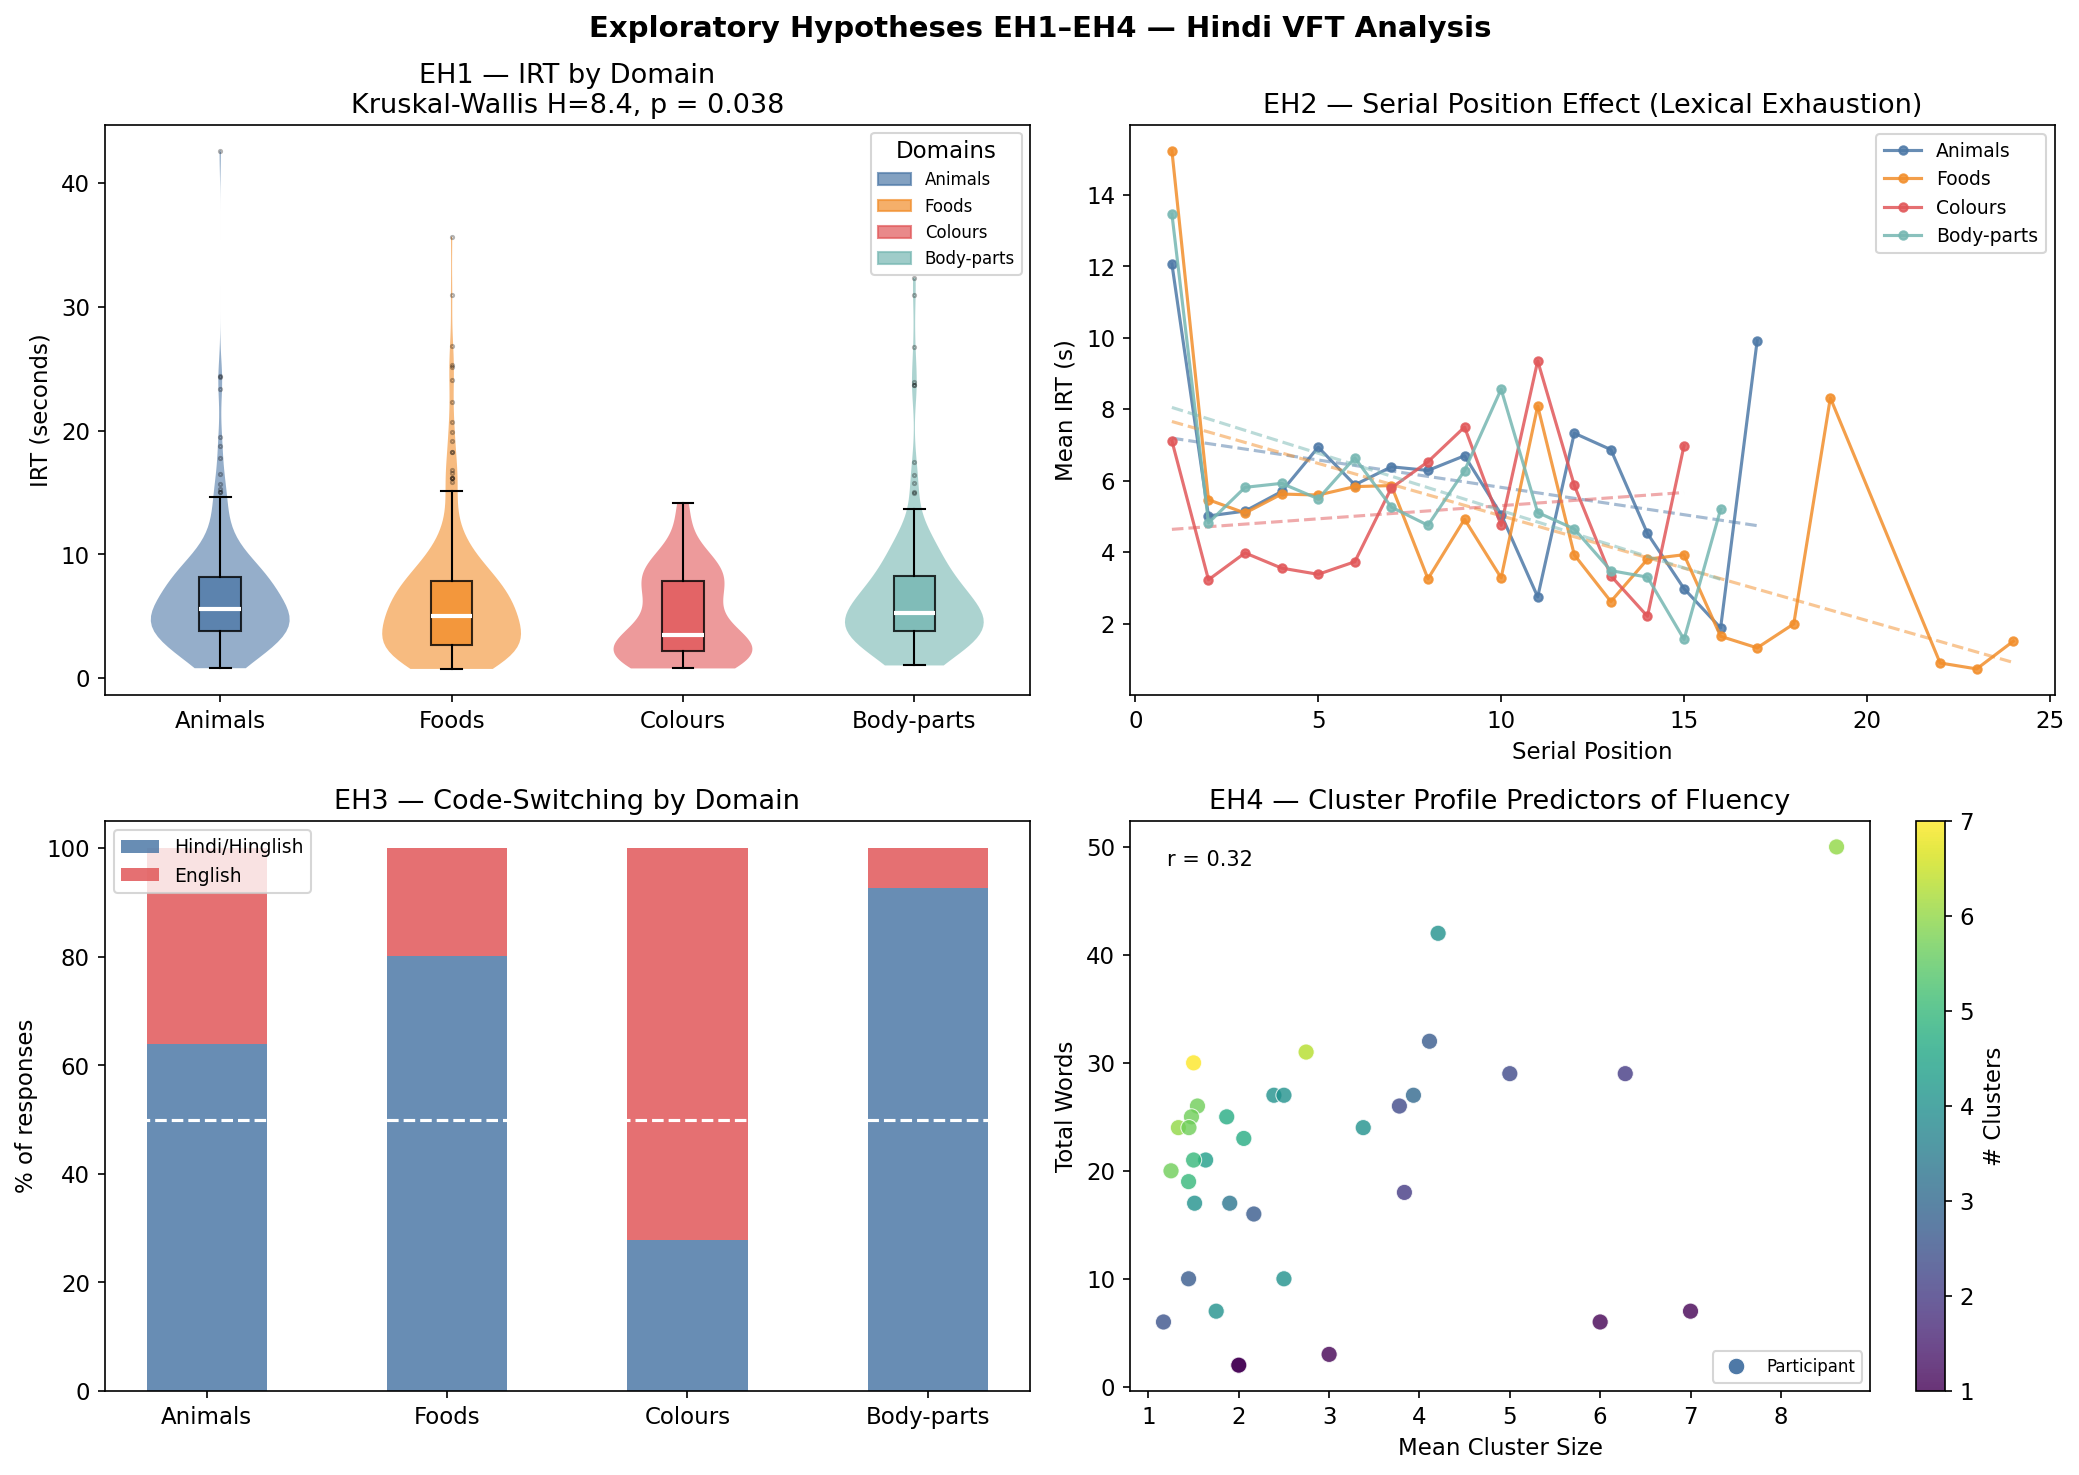
\includegraphics[keepaspectratio,alt={EH panel}]{images/eh1_eh4_panel.png}}
\caption{EH panel}
\end{figure}

\section{Transformer and Semantic Visual
Analysis}\label{transformer-and-semantic-visual-analysis}

\subsection{Embedding Visuals}\label{embedding-visuals}

These plots show semantic structure learned by transformer embeddings.

\begin{figure}
\centering
\pandocbounded{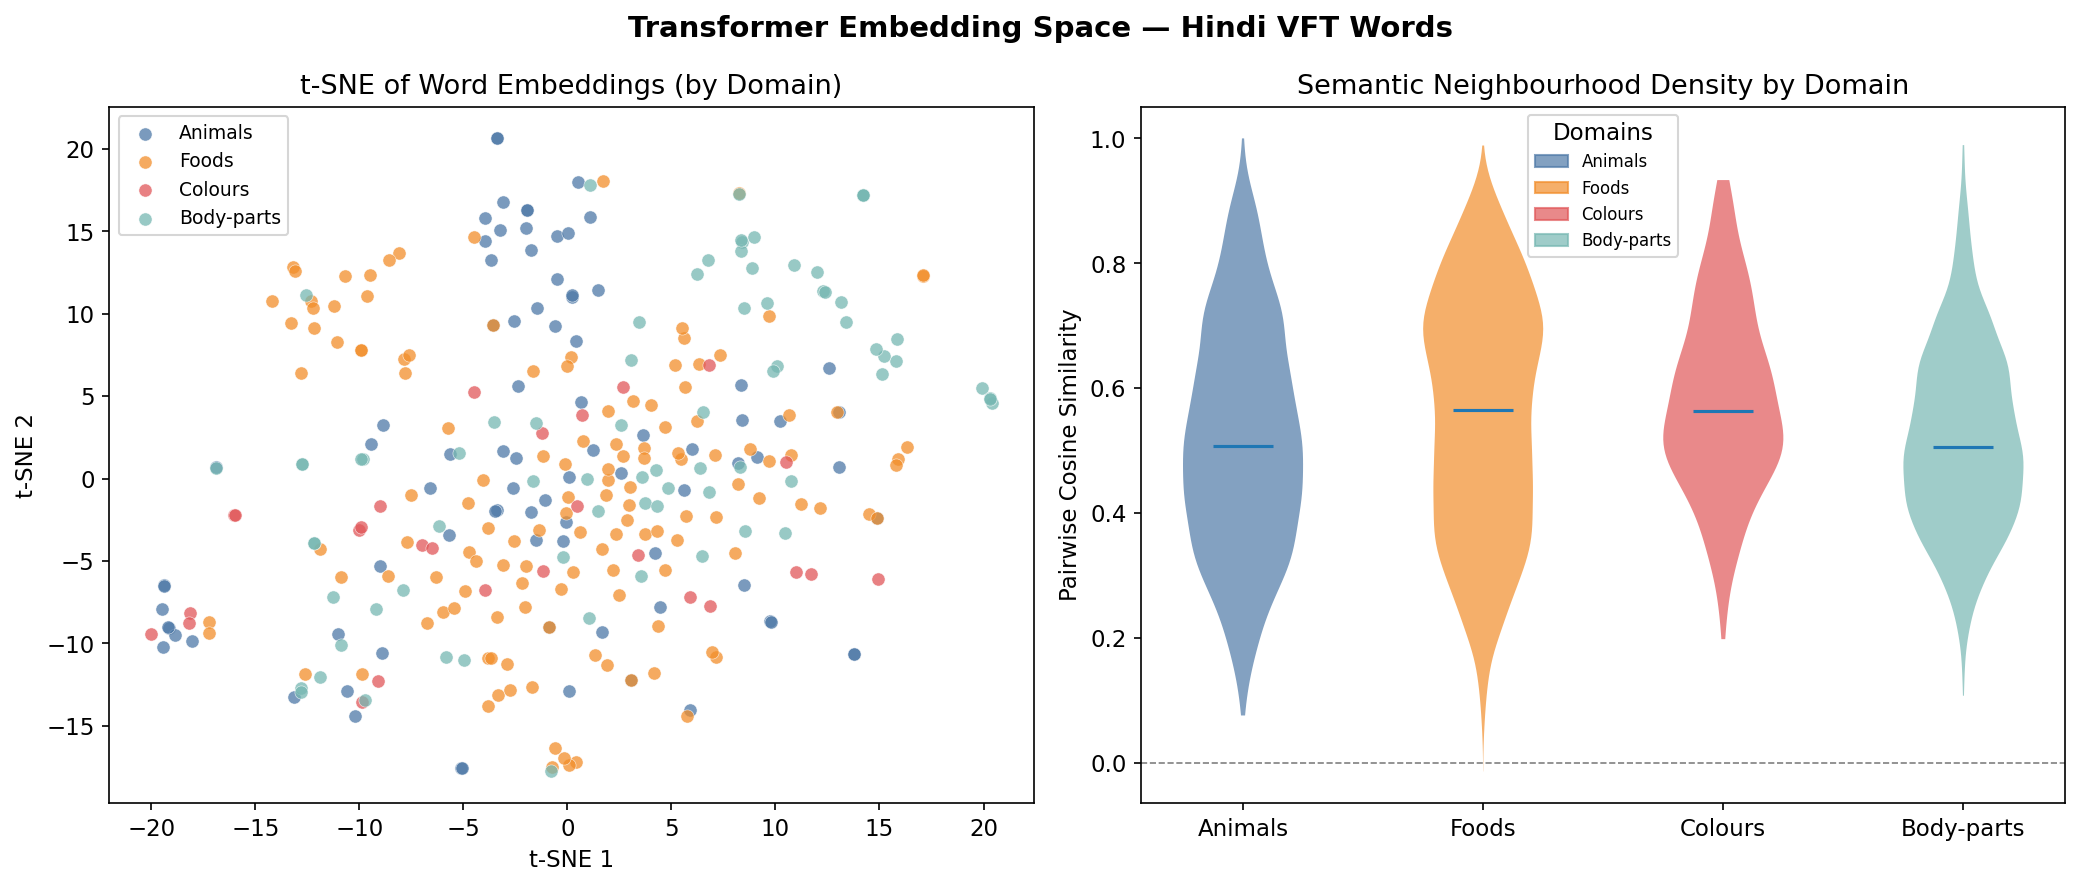
\includegraphics[keepaspectratio,alt={Embedding tSNE and similarity}]{images/embedding_tsne_similarity.png}}
\caption{Embedding tSNE and similarity}
\end{figure}

\begin{figure}
\centering
\pandocbounded{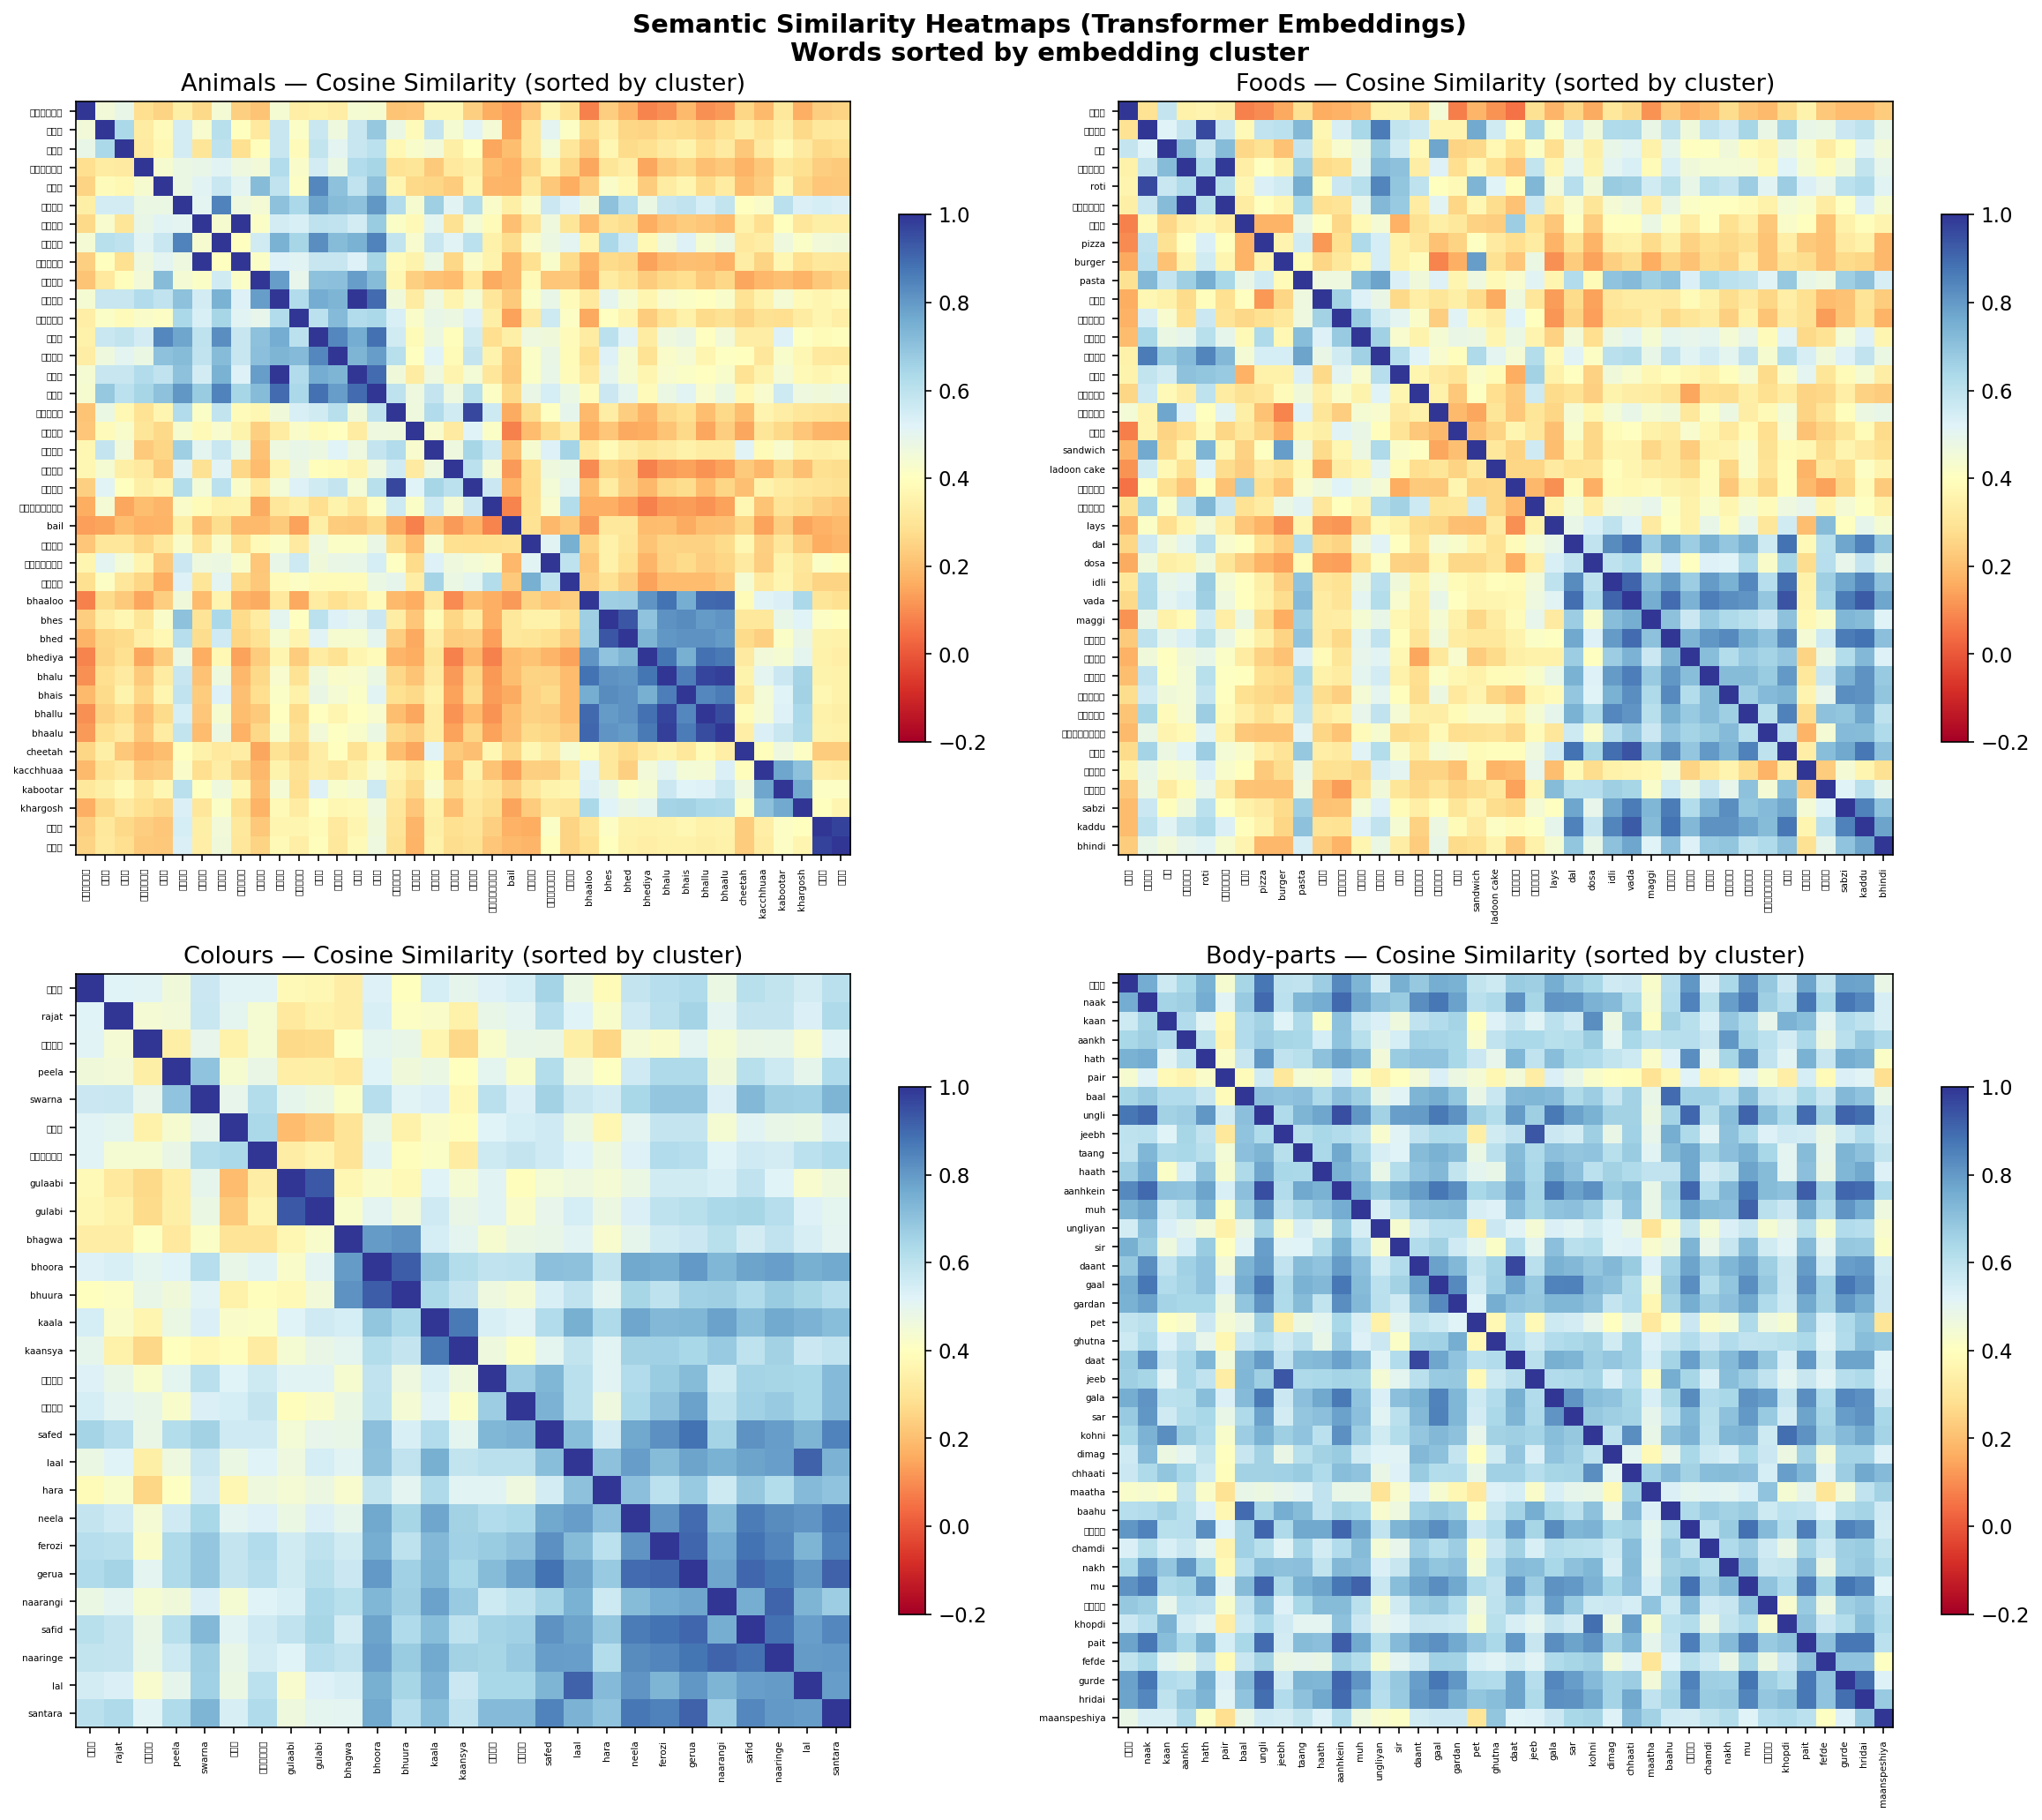
\includegraphics[keepaspectratio,alt={Embedding similarity heatmaps}]{images/similarity_heatmaps_emb.png}}
\caption{Embedding similarity heatmaps}
\end{figure}

\subsection{SpAM Spatial Visuals}\label{spam-spatial-visuals}

These plots show consensus semantic maps from participant placements.

\begin{figure}
\centering
\pandocbounded{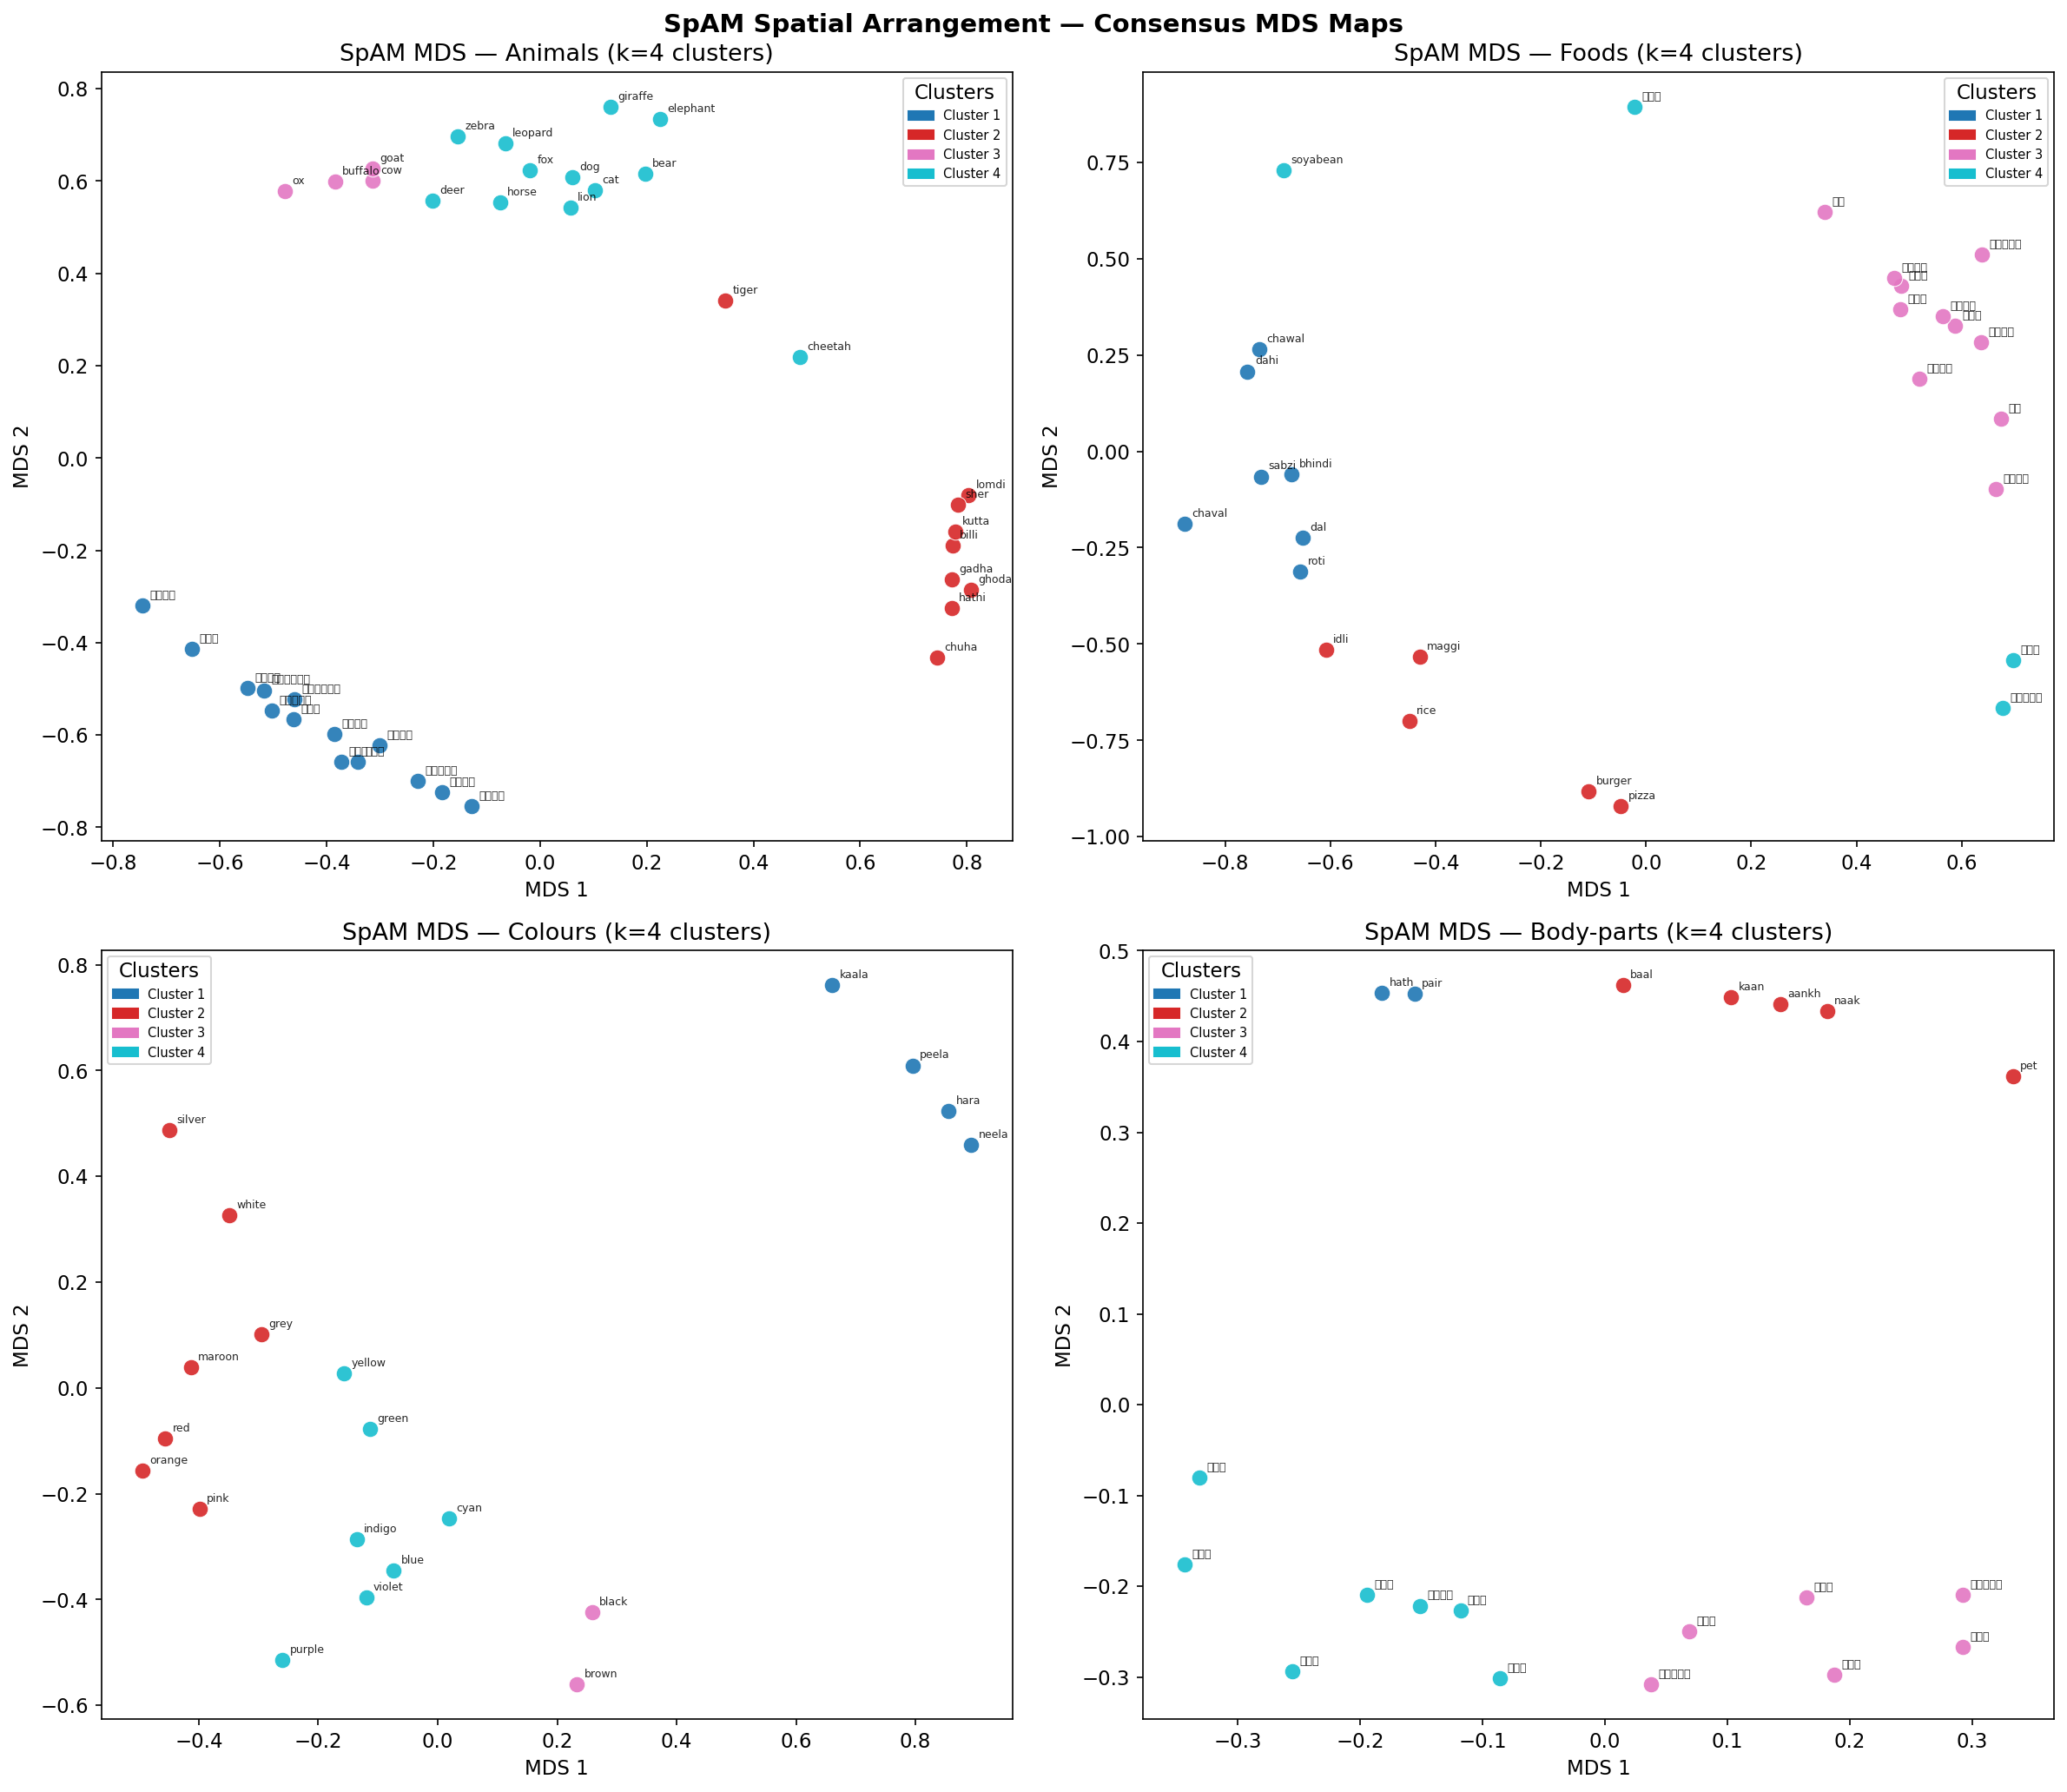
\includegraphics[keepaspectratio,alt={SpAM MDS consensus}]{images/spam_mds_consensus.png}}
\caption{SpAM MDS consensus}
\end{figure}

\section{Summary Table}\label{summary-table}

{\def\LTcaptype{none} % do not increment counter
\begin{longtable}[]{@{}
  >{\raggedright\arraybackslash}p{(\linewidth - 6\tabcolsep) * \real{0.2308}}
  >{\raggedright\arraybackslash}p{(\linewidth - 6\tabcolsep) * \real{0.2308}}
  >{\raggedleft\arraybackslash}p{(\linewidth - 6\tabcolsep) * \real{0.3077}}
  >{\raggedright\arraybackslash}p{(\linewidth - 6\tabcolsep) * \real{0.2308}}@{}}
\toprule\noalign{}
\begin{minipage}[b]{\linewidth}\raggedright
Item
\end{minipage} & \begin{minipage}[b]{\linewidth}\raggedright
Main test
\end{minipage} & \begin{minipage}[b]{\linewidth}\raggedleft
Result
\end{minipage} & \begin{minipage}[b]{\linewidth}\raggedright
Decision
\end{minipage} \\
\midrule\noalign{}
\endhead
\bottomrule\noalign{}
\endlastfoot
RQ1 & Wilcoxon signed rank & p = 0.368 & Not significant \\
RQ2 & Spearman correlation & p = 0.003 & Significant \\
RQ3 & Spearman correlation & p \textless{} .001 & Significant \\
RQ4 & Kruskal Wallis & p \textless{} .001 & Domains differ \\
RQ5 & Spearman and MixedLM & p = 0.954 & Not significant \\
EH1 & Kruskal Wallis & p \textless{} .001 & Domains differ \\
EH2 & Mixed model and domain slopes & Mixed & Position effect exists \\
EH3 & Proportion comparison & Mixed & Domain specific \\
EH4 & Spearman correlation & p = 0.0026 for cluster size & Significant
for cluster size \\
\end{longtable}
}

\section{Discussion}\label{discussion}

This final analysis follows strict normality-first test selection. That
keeps statistical decisions consistent.

Supported findings are RQ2 RQ3 and RQ4. Not supported findings are RQ1
and RQ5.

Main practical story is:

\begin{enumerate}
\def\labelenumi{\arabic{enumi}.}
\tightlist
\item
  Better clustering is linked to better fluency.
\item
  Cross-task semantic signal is strongest in Animals.
\item
  Domain effects are strong in timing and compactness.
\item
  Transformer semantics and human semantic arrangement both show domain
  dependence.
\end{enumerate}

\section{Conclusion}\label{conclusion}

This final report gives one complete picture from VFT and SpAM together.
Methodology stayed consistent with normality-first test selection. This
improves reliability of inference.

From confirmatory questions:

\begin{enumerate}
\def\labelenumi{\arabic{enumi}.}
\tightlist
\item
  RQ2 is supported and shows useful clustering effect on fluency.
\item
  RQ3 is supported overall with strongest signal in Animals.
\item
  RQ4 is supported and confirms domain-wise compactness difference.
\item
  RQ1 and RQ5 are not supported in this sample.
\end{enumerate}

From exploratory checks:

\begin{enumerate}
\def\labelenumi{\arabic{enumi}.}
\tightlist
\item
  Domain effect on timing is strong.
\item
  Serial position effect is present but domain dependent.
\item
  Code-switching behavior is domain specific.
\item
  Cluster size is strongest cluster metric for fluency.
\end{enumerate}

Overall meaning in simple words is this. Hindi semantic retrieval is
structured and domain dependent. SpAM and VFT together give a useful
combined view. Transformer-based semantic features and human semantic
judgments both support this.

\section{References}\label{references}

\begin{thebibliography}{9}

\bibitem{troyer1997}
Troyer, A. K., Moscovitch, M., and Winocur, G. (1997).
Clustering and switching as two components of verbal fluency.
    extit{Neuropsychology}, \textit{11}(1), 138-146.

\bibitem{hills2012}
Hills, T. T., Jones, M. N., and Todd, P. M. (2012).
Optimal foraging in semantic memory.
    extit{Psychological Review}, \textit{119}(2), 431-440.

\bibitem{hout2013}
Hout, M. C., Goldinger, S. D., and Ferguson, R. W. (2013).
The versatility of SpAM.
    extit{Journal of Experimental Psychology: General}, \textit{142}(1), 256-281.

\bibitem{benjamini1995}
Benjamini, Y., and Hochberg, Y. (1995).
Controlling the false discovery rate.
    extit{Journal of the Royal Statistical Society: Series B}, \textit{57}(1), 289-300.

\bibitem{bhatt2022}
Bhatt, R., Anderson, N. D., and Bhatt, M. (2022).
Verbal fluency in bilingual South Asian older adults.
    extit{Journal of the International Neuropsychological Society}, \textit{28}(4), 412-421.

\bibitem{kumar2022}
Kumar, A., Lundin, N. B., and Jones, M. N. (2022).
Mouse-Mole-Vole: The Inconspicuous Benefit of Phonology During Retrieval from Semantic Memory.
    extit{PsyArXiv}. DOI: 10.31234/osf.io/2bazx.

\bibitem{dautriche2016}
Dautriche, I., Mahowald, K., Gibson, E., and Piantadosi, S. T. (2016).
Wordform Similarity Increases With Semantic Similarity: An Analysis of 100 Languages.
    extit{Cognitive Science}, 1-21. DOI: 10.1111/cogs.12453.

\end{thebibliography}
